\section{Géométrie spatiale}

\subsection{Règles de la perspective cavalière}

\begin{itemize}
\item[*] Une droite de l'espace est représentée par une droite.
\item[*] Deux droites parallèles de l'espace sont représentées par deux droites parallèles.
\item[*] Le milieu d'un segment de l'espace est représenté au milieu du segment.
\item[*] Les éléments visibles sont dessinés en trains pleins et les éléments cachés en pointillés.
\item[*] Dans un plan vu de face, les éléments sont représentés en vraie grandeur.
\end{itemize}

\subsection{Les solides usuels}

\subsubsection{Les solides droits.}

% Dessins plus texte.

\begin{center}
\begin{tabular}{l@{$\quad$}|@{$\quad$}l|@{$\quad$}l@{$\quad$}|l}
\multicolumn{1}{c@{$\quad$}|@{$\quad$}}{\bf Le pavé droit} & 
      \multicolumn{2}{c}{\bf Les prismes} & 
          \multicolumn{1}{|c}{\bf Le cylindre } \\
   & $\mathrm{Ex}_1$     & $\mathrm{Ex}_2$ & \\    
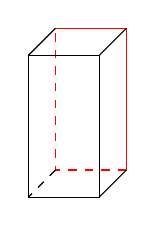
\begin{tikzpicture}[scale=.9]  % ------ Le pavé-----------------------------
      [x={(-0.572cm,-0.416cm)},y={(1cm,0cm)},z={(0cm,1cm)}]
    \draw [dashed, red] (1,0,0)--(0,0,0) --(0,2,0) ;
    \draw [red] (0,2,0)--(1,2,0)--(1,2,0)-- (1,0,0);
    \draw (0,0,1)--(1,0,1)--(1,2,1)--(0,2,1)--cycle;
    \draw [dashed] (0,0,0)--(0,0,1) ;
    \draw (1,0,0)--(1,0,1);
    \draw (0,2,0)--(0,2,1);
    \draw (1,2,0)--(1,2,1);
\end{tikzpicture} 
& 
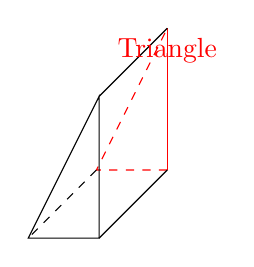
\begin{tikzpicture}[scale=.9] % ------ Le prisme triangle -----------------
      [x={(-0.572cm,-0.416cm)},y={(1cm,0cm)},z={(0cm,1cm)}]
    \draw [dashed, red] (1,0,0)--(0,0,0)--(1,2,0);
    \draw [red] (1,2,0) -- (1,0,0) ; 
    \draw (0,0,2.5)--(1,0,2.5)--(1,2,2.5)--cycle;
    \draw [dashed] (0,0,0)--(0,0,2.5);
    \draw (1,0,0)--(1,0,2.5);
    \draw (1,2,0)--(1,2,2.5);
    \draw [red] (1,2,0) node [below] {Triangle} ; 
\end{tikzpicture}
& 
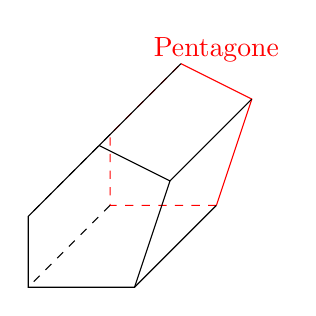
\begin{tikzpicture}[scale=.9] % ------ Le prisme pentagone ----------------
      [x={(-0.572cm,-0.416cm)},y={(1cm,0cm)},z={(0cm,1cm)}]
    \draw [dashed,red](1.5,0,0)--(0,0,0)--(0,1,0)--(1,2,0); 
    \draw [red] (1,2,0) -- (2,1.5) -- (1.5,0,0) ; 
    \draw (0,0,3)--(0,1,3)--(1,2,3)--(2,1.5,3)--(1.5,0,3)--cycle ;
    \draw [dashed] (0,0,0)--(0,0,3);
    \draw [dashed] (0,1,0)--(0,1,3);
    \draw (1,2,0)--(1,2,3);
    \draw (2,1.5,0)--(2,1.5,3);
    \draw (1.5,0,0)--(1.5,0,3);
    \draw [red] (1.5,2.5,0) node [below] {Pentagone} ; 
\end{tikzpicture}
& 
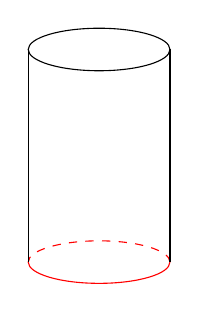
\begin{tikzpicture}[scale=.9] % ------ Le cylindre --------------------
\draw [red] (-1,0) arc (180:360:1 and .3) ;
\draw [dashed, red] (1,0) arc (0:180:1 and .3) ;
\draw (0,3)  circle  (1 and .3); 
\draw (-1,0) -- (-1,3) ; 
\draw (1,0) -- (1,3) ; 
\end{tikzpicture} \\
 & 
      \multicolumn{2}{c}{La base est un polygone} & 
          \multicolumn{1}{c}{\textcolor{red}{La base est un disque}} \\
\multicolumn{4}{l}{$V=\beta \times h. \qquad \begin{array}{l}
                              \beta=\mathrm{Aire\;de\;la\;base}\\
                                          h = \mathrm{hauteur}
                                          \end{array}$} \\      
\end{tabular}
\end{center}


\subsubsection{Les pyramides et les cônes}

%Dessins plus texte.

\begin{center}
\begin{tabular}{l@{$\quad$}|@{$\quad$}l|@{$\quad$}l@{$\quad$}|l}
\multicolumn{1}{c@{$\quad$}|@{$\quad$}}{\bf Le tétraèdre} & 
      \multicolumn{2}{c}{\bf Les pyramides} & 
          \multicolumn{1}{|c}{\bf Le cylindre } \\
   & $\mathrm{Ex}_1$     & $\mathrm{Ex}_2$ & \\     
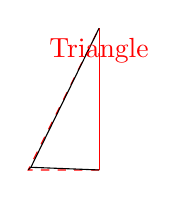
\begin{tikzpicture} [scale=.9]% ------ Tétraèdre -----------------
      [x={(-0.572cm,-0.416cm)},y={(1cm,0cm)},z={(0cm,1cm)}]
    \draw [dashed, red] (1,0,0)--(0,0,0)--(1,2,0);
    \draw [red] (1,2,0) -- (1,0,0) ; 
    \draw [dashed] (0,0,0)--(1,1,2.5);
    \draw (1,0,0)--(1,1,2.5);
    \draw (1,2,0)--(1,1,2.5);
    \draw [red] (1,2,0) node [below] {Triangle} ; 
\end{tikzpicture}  &
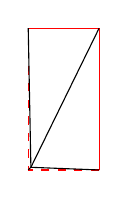
\begin{tikzpicture} [scale=.9] % ------ Pyramide N°1-----------------------------
      [x={(-0.572cm,-0.416cm)},y={(1cm,0cm)},z={(0cm,1cm)}]
    \draw [dashed, red] (1,0,0)--(0,0,0) --(0,2,0) ;
    \draw [red] (0,2,0)--(1,2,0)--(1,2,0)-- (1,0,0);
    \draw [dashed] (0,0,0)--(1,1,2.5) ;
    \draw (1,0,0)--(1,1,2.5);
    \draw (0,2,0)--(1,1,2.5);
    \draw (1,2,0)--(1,1,2.5);
\end{tikzpicture} 
& 
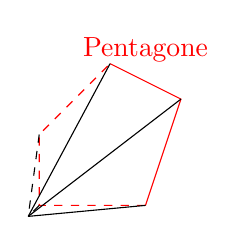
\begin{tikzpicture} [scale=.9]% ------ Pyramide N°2 ----------------
      [x={(-0.572cm,-0.416cm)},y={(1cm,0cm)},z={(0cm,1cm)}]
    \draw [dashed,red](1.5,0,0)--(0,0,0)--(0,1,0)--(1,2,0); 
    \draw [red] (1,2,0) -- (2,1.5) -- (1.5,0,0) ; 
    \draw [dashed] (0,0,0)--(1,1,3);
    \draw [dashed] (0,1,0)--(1,1,3);
    \draw (1,2,0)--(1,1,3);
    \draw (2,1.5,0)--(1,1,3);
    \draw (1.5,0,0)--(1,1,3);
    \draw [red] (1.5,2.5,0) node [below] {Pentagone} ; 
\end{tikzpicture}
& 
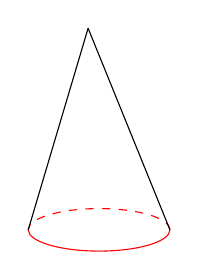
\begin{tikzpicture}[scale=.9] % ------ Le cône --------------------
\draw [red] (-1,0) arc (180:360:1 and .3) ;
\draw [dashed, red] (1,0) arc (0:180:1 and .3) ;
\draw (-1,0,0) -- (1,4,3) ; 
\draw (1,0,0) -- (1,4,3) ; 
\end{tikzpicture} \\
 & 
      \multicolumn{2}{c}{La base est un polygone} & 
          \multicolumn{1}{c}{\textcolor{red}{La base est un disque}} \\
\multicolumn{4}{l}{$V=\dfrac{1}{3}\beta \times h$} \\      
\end{tabular}
\end{center}

\subsubsection{La sphère}

%Dessins plus texte.
\begin{center}
  \begin{tikzpicture}[scale=.9]
    \coordinate (O) at (0,0) ;
    \draw[thin,gray] (O) circle (2cm) ;
    \draw[red,rotate=35,dashed] (O) ellipse (2 and 1) ;
    \draw (O) node {\large $\times$} ; 
    \draw (O) -- (-1,0) node [above] {r = rayon} -- (-2,0)  ; 
    \draw (3,0) node {$V=\dfrac{4}{3}\pi r^3$} ; 
  \end{tikzpicture}
\end{center}

\newpage 

\subsection{Exercice}

%dessin

\begin{tabular}{cc}

%----------- Tétraèdre 

\begin{tikzpicture}[line cap=round,line join=round,>=triangle 45, x={(-0.572cm,-0.416cm)},y={(1cm,0cm)},z={(0cm,1cm)}]
\draw  [dashed] (0,0,0)-- (-1.12,-2.78,0);
\draw  [dashed]  (-1.12,-2.78,0)-- (1.85,-2.36,0);
\draw  (1.85,-2.36,0)-- (0,0,0);
\draw [dashed] (0.22,-1.72,0)-- (-.7,-1.8,0);
\draw (0,0,0)-- ++(-1.0pt,-1.0pt) -- ++(2.0pt,2.0pt) ++(-2.0pt,0) -- ++(2.0pt,-2.0pt);
\draw  [dashed] (0.22,-1.72,0) -- (0.22,-1.72,2.5) ; 
\draw  (0,0,0) -- (0.22,-1.72,2.5) ; 
\draw  [dashed] (-1.12,-2.78,0) -- (0.22,-1.72,2.5) ; 
\draw  (1.85,-2.36,0) -- (0.22,-1.72,2.5) node [above] {$A$} ; 
\draw(-0.24,0.1,0)   node {$C$};
\draw(-1.5,-3,0) node [left] {$D$}; 
\draw (2,-2.3,0)    node [left] {$B$};
\draw(0.38,-1.5,0)   node [left] {$H$};
\draw(-1.2,-2.2,0)  node [right] {$E$};
\end{tikzpicture} & 
\raisebox{10ex}{\parbox {11cm}{
Soit ABCD un tétraèdre régulier. Les quatres faces sont des triangles équilatéraux. On a $AB = BC = CA = AD = DC = BD = a$. \\

H est le pied de la hauteur issue de $A$. $H$ est ainsi le centre de gravité du triangle $BCD$ car $BCD$ est un triangle équilatéral. \\

E est le point d'intersection de $\left(BH\right)$ et de $\left(CD\right)$. E est le milieu de $\left[CD\right]$ car $ \left(BH\right)$ est une médiane du triangle $BCD$. Le triangle $BEC$ est rectangle en E car $\left(BH\right)$ est aussi une hauteur du triangle $BCD$. }}\\

\end{tabular}

\subsubsection*{Théorème de Pythagore dans le triangle BEC rectangle en E}

$ BE^2 + EC^2 = BC^2$ \\

$ BE^2 + \left(\dfrac{1}{2}a\right)^2 = a^2$ \\

$ BE^2 + \dfrac{1}{4}a^2 = a^2$ \\

$ BE^2 =a^2 - \dfrac{1}{4}a^2$ \\

$ BE^2 = \dfrac{3}{4}a^2 $ \\

$ BE = \sqrt{\dfrac{3}{4} a^2} = \dfrac{a\sqrt{3}}{2} $ \\

D'autre part, $ BH = \dfrac{2}{3} BE $, d'où $BH = \dfrac{2}{3} \times \dfrac{a\sqrt{3}}{2} $. \\

Ainsi, $BH = \dfrac{a\sqrt{3}}{3}$ \\

\newpage

\subsubsection*{Le triangle AHB est rectangle en H}

$ AH^2 + BH^2 = AB^2 $ \\

$ AH^2 + \left(\dfrac{a\sqrt{3}}{3}\right)^2 = a^2$ \\

$ AH^2 + \dfrac{a^2}{3} = a^2$ \\

$ AH^2 =a^2 - \dfrac{a^2}{3}$ \\

$ AH^2 = \dfrac{2}{3}a^2 $ \\

$ AH = \sqrt{\dfrac{2a^2}{3}} = \dfrac{a\sqrt{2}}{\sqrt{3}} = \dfrac{a\sqrt{6}}{3} $ \\

\subsubsection*{Aire de la base = aire du triangle BCD}

$\beta = \dfrac{1}{2} CD \times BE$ \\

$\beta = \dfrac{1}{2} a \times \dfrac{a\sqrt{3}}{2}$ \\

$ \beta = a^2 \dfrac{\sqrt{3}}{4} $ \\

Soit $V$ le volume de $ABCD$. On a $h = AH$ et $\beta =$ aire de $BCD$. \\

$ V = \dfrac{1}{3}\beta \times h $ \\

$ V = \dfrac{1}{3} \times a^2\dfrac{\sqrt{3}}{4} \times \dfrac{a\sqrt{6}}{3} $ \\

$ V = a^3 \times \dfrac{\sqrt{18}}{36} $ \\

$ V = a^3 \dfrac{3\sqrt{2}}{36} $ \\

$ V = \dfrac{a^3\sqrt{2}}{12} $ \\

\newpage

\subsection{Calcul du nombre d'arêtes d'un solide convexe}

Euler a établi que tous les solides convexes vérifient la formule : $S + F - A = 2 $.

\subsubsection*{Ballon de football}


\begin{tabular}{cl}
\raisebox{4ex}{\parbox{8cm}{
12 pentagones et 20 hexagones réguliers.

\begin{itemize}
\item[*] S = 60 ($12 \times 5$)
\item[*] F = 32 (20 + 12)
\item[*] A = 90
\end{itemize}}} & 
\includegraphics[width=.1\textwidth]{Ballon-de-football.jpeg}\\
\end{tabular}
\subsection{Les solides de Platon}

Il existe cinq polyèdres réguliers convexes inscriptibles dans une sphère.

\subsubsection{Tétraèdre}

Quatre triangles équilatéraux.

% Dessin

\begin{center}


\begin{tabular}{cc}
    \begin{tikzpicture}[line cap=round,line join=round,>=triangle 45,             
            x={(-0.572cm,-0.416cm)},y={(1cm,0cm)},z={(0cm,1cm)}]
        \draw  [dashed] (0,0,0)-- (-1.12,-2.78,0);                % DC 
        \draw  [dashed]  (-1.12,-2.78,0)-- (1.85,-2.36,0);        % DB 
        \draw  (1.85,-2.36,0)-- (0,0,0);                          % BC
        \draw  (0,0,0) -- (0.22,-1.72,2.5) ;                      % AC 
        \draw  [dashed] (-1.12,-2.78,0) -- (0.22,-1.72,2.5) ;     % AD 
        \draw  (1.85,-2.36,0) -- (0.22,-1.72,2.5) ;               % AB node [above] {$A$} ; 
    \end{tikzpicture} & \raisebox{10ex}{\parbox{4cm}{
        \begin{itemize}
            \item[*] $S = 4$
            \item[*] $F = 4$
            \item[*] $A = 6$
        \end{itemize}}}\\
\end{tabular}

\end{center}

Il représentait l'élément feu.

\subsubsection{Cube}

Six carrés.

% Dessin

\begin{center}

\begin{tabular}{cc}
\raisebox{10ex}{\parbox{4cm}{
        \begin{itemize}
            \item[*] $S = 8$
            \item[*] $F = 6$
            \item[*] $A = 12$
        \end{itemize}}} & 
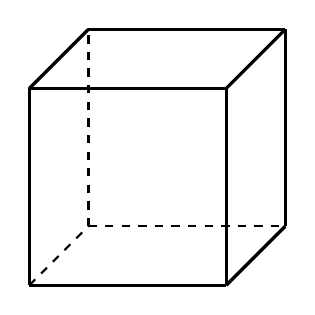
\begin{tikzpicture}[thick,scale=2.5]
    \coordinate (A1) at (0, 0);
    \coordinate (A2) at (0, 1);
    \coordinate (A3) at (1, 1);
    \coordinate (A4) at (1, 0);
    \coordinate (B1) at (0.3, 0.3);
    \coordinate (B2) at (0.3, 1.3);
    \coordinate (B3) at (1.3, 1.3);
    \coordinate (B4) at (1.3, 0.3);

    \draw[very thick] (A1) -- (A2);
    \draw[very thick] (A2) -- (A3);
    \draw[very thick] (A3) -- (A4);
    \draw[very thick] (A4) -- (A1);

    \draw[dashed] (A1) -- (B1);
    \draw[dashed] (B1) -- (B2);
    \draw[very thick] (A2) -- (B2);
    \draw[very thick] (B2) -- (B3);
    \draw[very thick] (A3) -- (B3);
    \draw[very thick] (A4) -- (B4);
    \draw[very thick] (B4) -- (B3);
    \draw[dashed] (B1) -- (B4);

%    \draw[fill=yellow,opacity=0.6] (A1) -- (B1) -- (B4) -- (A4);
%    \draw[fill=black!20,opacity=0.5] (A1) -- (A2) -- (A3) -- (A4);
%    \draw[fill=red,opacity=0.6] (A1) -- (A2) -- (B2) -- (B1);
%    \draw[fill=black,opacity=0.6] (B1) -- (B2) -- (B3) -- (B4);
%    \draw[fill=blue,opacity=0.6] (A3) -- (B3) -- (B4) -- (A4);
%    \draw[fill=green,opacity=0.6] (A2) -- (B2) -- (B3) -- (A3);

\end{tikzpicture} \\
\end{tabular}
\end{center}

Il représentait l'élément terre.

\newpage

\subsubsection{Octaèdre}

Huit triangles équilatéraux.

% Dessin
\begin{center}

\begin{tabular}{cc}
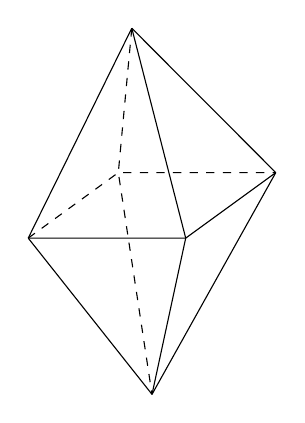
\begin{tikzpicture}  % ------ L'octaèdre-----------------------------
      [x={(-0.572cm,-0.416cm)},y={(1cm,0cm)},z={(0cm,1cm)}, scale=2]
      
    \coordinate (A1) at (0,0,0);    
    \coordinate (A2) at (0,1,0);
    \coordinate (A3) at (1,1,0);  
    \coordinate (A4) at (1,0,0);  
    \coordinate (B1) at (.2,.2,1);
    \coordinate (B2) at (.5,.5,-1.2);  


%     \draw [dashed] (A4) node {A2} -- (A1) node {A1}  --(A2) node {A2} ; % pour debug 
    \draw [dashed] (A4) -- (A1)  -- (A2)  ; 
    \draw  (A2)--(A3)--(A4);
    \draw  [dashed] (B1)--(A1) --(B2); 
    \draw  (A2)--(B1); \draw  (A3)--(B1);  \draw  (A4)--(B1);
 \draw  (A2)--(B2); \draw  (A3)--(B2);  \draw  (A4)--(B2);  
    
\end{tikzpicture} & 
\raisebox{10ex}{\parbox{4cm}{
        \begin{itemize}
            \item[*] $S = 6$
            \item[*] $F = 8$
            \item[*] $A = 12$
        \end{itemize}}}
\end{tabular}
\end{center}

Il représentait l'élément air.

\subsubsection{Dodécaèdre}

12 pentagones réguliers.

\begin{center}

\begin{tabular}{cc}
\raisebox{10ex}{\parbox{4cm}{
        \begin{itemize}
            \item[*] $S = 20$
            \item[*] $F = 12$
            \item[*] $A = 30$
        \end{itemize}}} & 
\includegraphics[width=.3\textwidth]{Docecaedre.jpg}\\
\end{tabular}
\end{center}

Il représentait l'univers.

\subsubsection{Icosaèdre}

30 triangles équilatéraux.

% Dessin
\begin{center}

\begin{tabular}{cc}
 \includegraphics[width=.3\textwidth]{icosaedre.jpg}& 
\raisebox{10ex}{\parbox{4cm}{
        \begin{itemize}
            \item[*] $S = 12$
            \item[*] $F = 20$
            \item[*] $A = 30$
        \end{itemize}}}
\end{tabular}
\end{center}

Il représentait l'eau.

\subsection{Détermination d'un plan}

\subsubsection{Axiome \no 1}

Il existe un plan $P$ et un seul, passant par 3 points A, B et C non-alignés. \\

%Dessin + légende

\begin{center}

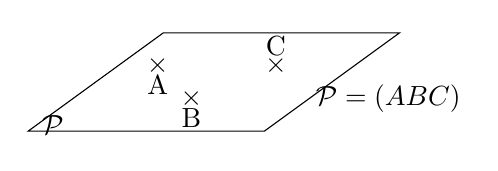
\begin{tikzpicture}  % ------ Trois points forment un plan --------------
      [x={(-0.572cm,-0.416cm)},y={(1cm,0cm)},z={(0cm,1cm)}, scale=1]
      
    \coordinate (P1) at (0,0,0);    
    \coordinate (P2) at (0,3,0);
    \coordinate (P3) at (3,3,0);  
    \coordinate (P4) at (3,0,0);  
    \coordinate (A) at (1,.5,0); 
    \coordinate (B) at (2,1.5,0);  
    \coordinate (C) at (1,2,0); 
    \coordinate (L) at (2,4,0); 
    

    \draw (P1)  -- (P2)  -- (P3) -- (P4) -- cycle  ; 
    \draw  (A) node {$\times$} ; \draw  (B) node  {$\times$} ; \draw  (C) node  {$\times$} ; 
    \draw  (A) node [below] {A} ; \draw (B)  node [below]  {B} ; \draw (C) [above]node  {C} ; 
    
    \draw (2.8,.2,0) node {$\mathcal{P}$} ;
    \draw (L) node {$\mathcal{P}=(ABC)$} ; 
\end{tikzpicture}
\end{center}

\subsubsection{Axiome \no 2}

Soient A et B deux points distincts d'un plan $P$. La droite $(AB)$ est entièrement contenue dans le plan. \\

% Dessin + légende
\begin{center}
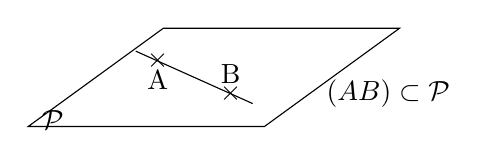
\begin{tikzpicture}  % ------ Une droite dans un plan -------------------
      [x={(-0.572cm,-0.416cm)},y={(1cm,0cm)},z={(0cm,1cm)}, scale=1]
      
    \coordinate (P1) at (0,0,0);    
    \coordinate (P2) at (0,3,0);
    \coordinate (P3) at (3,3,0);  
    \coordinate (P4) at (3,0,0);  
    \coordinate (A) at (1,.5,0); 
    \coordinate (B) at (2,2,0); 
    \coordinate (L) at (2,4,0); 
    

    \draw (P1)  -- (P2)  -- (P3) -- (P4) -- cycle  ; 
    \draw  (A) node {$\times$} ; \draw  (B) node  {$\times$}  ; 
    \draw  (A) node [below] {A} ; \draw (B)  node [above ]  {B} ; 
    \draw (.7,.05,0) -- (2.3,2.45,0)  ; % (AB) 1.5x -1 
    \draw (2.8,.2,0) node {$\mathcal{P}$} ;
    \draw (L) node {$(AB) \subset \mathcal{P}$} ; 
\end{tikzpicture}
\end{center}

\subsubsection{Conclusion}

Compte-tenu des deux axiomes précédents, un plan est difini par : 
\begin{itemize}
\item Trois points \textbf{non alignés}
\item Deux droites sécantes $D_1$ et $D_2$.
%dessin

\begin{center}
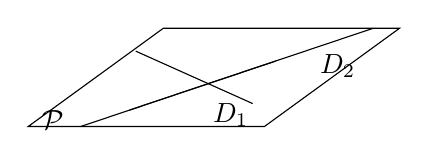
\begin{tikzpicture}  % ------ Deux droites secantes dans un plan --------
      [x={(-0.572cm,-0.416cm)},y={(1cm,0cm)},z={(0cm,1cm)}, scale=1]
      
    \coordinate (P1) at (0,0,0);    
    \coordinate (P2) at (0,3,0);
    \coordinate (P3) at (3,3,0);  
    \coordinate (P4) at (3,0,0);  
    \coordinate (A) at (1,.5,0); 
    \coordinate (B) at (2,2,0); 
    \coordinate (C) at (.5,2.5,0); 
    \coordinate (L) at (2,4,0); 
    

    \draw (P1)  -- (P2)  -- (P3) -- (P4) -- cycle  ; 
    \draw  (C) node [below] {$D_2$} ; \draw  (B) node  [below] {$D_1$}  ; 
    \draw (.7,.05,0) -- (2.3,2.45,0) ;  % (AB)  = 1.5x-1 
    \draw (1,2,0) -- (2.5,1,0) ;  % (CB)  = (-2/3)x +(8/3)  
    \draw (0,8/3,0) -- (3,2/3,0)  ; 
    \draw (2.8,.2,0) node {$\mathcal{P}$} ;
\end{tikzpicture}
\end{center}

\item Deux droites parallèes $D_1$ et $D_2$.
%dessin.
\begin{center}
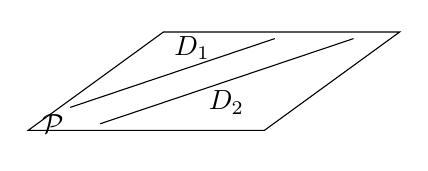
\begin{tikzpicture}  % ------ Deux droites parallèles dans un plan -------
      [x={(-0.572cm,-0.416cm)},y={(1cm,0cm)},z={(0cm,1cm)}, scale=1]
      
    \coordinate (P1) at (0,0,0);    
    \coordinate (P2) at (0,3,0);
    \coordinate (P3) at (3,3,0);  
    \coordinate (P4) at (3,0,0);  
    \coordinate (A) at (1,.5,0); 
    \coordinate (B) at (2,2,0); 
    \coordinate (C) at (.5,2.5,0); 
    \coordinate (L) at (2,4,0); 
    

    \draw (P1)  -- (P2)  -- (P3) -- (P4) -- cycle  ; 
  \draw  (1.5,1.66,0) node [below] {$D_2$} ;  \draw  (.5,1,0) node  [left] {$D_1$}  ; 
    \draw (.2,1.53,0)   -- (2.3,0.133,0);  % (D1)  = (-2/3)x +(5/3) 
    \draw (.2,2.53,0)-- (2.8,.8,0) ;  % (D2)  = (-2/3)x +(8/3)  
    \draw (2.8,.2,0) node {$\mathcal{P}$} ;
\end{tikzpicture}
\end{center}
\end{itemize}

\subsubsection{Définition}

\begin{itemize}
\item[*] 4 points de l'espace sont \underline{coplanaires} s'ils appartiennent à un même plan.
\item[*] 2 droites de l'espace sont coplanaires si et seulement si elles sont incluses dans un même plan.
\item[*] Deux droites $D_1$ et $D_2$ sont coplanaires si et seulement si $D_1$ et $D_2$ sont \textbf{soit} sécantes \textbf{soit} parallèles.
\item[*] Deux droites $D_1$ et $D_2$ sont non coplanaires si et seulement si $D_1$ et $D_2$ sont \textbf{ni} sécantes \textbf{ni} parallèles.
\end{itemize}

\subsection{Position relative dans l'espace}

\subsubsection{Position relative de deux droites}

%dessin + textes.

\begin{center}
\begin{tabular}{cccc}
\multicolumn{1}{c}{$D_1$ et $D_2$ sont sécantes} &
       \multicolumn{2}{c}{$D_1$ et $D_2$ sont parallèles} &
              \multicolumn{1}{c}{$D_1$ et $D_2$ sont} \\
\multicolumn{3}{c}{} &  \multicolumn{1}{c}{ non-coplanaires} \\             
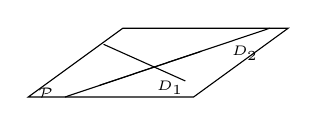
\begin{tikzpicture}  % ------ Deux droites secantes dans un plan --------
      [x={(-0.572cm,-0.416cm)},y={(1cm,0cm)},z={(0cm,1cm)}, scale=.7]
\begin{tiny}    
    \coordinate (P1) at (0,0,0);    
    \coordinate (P2) at (0,3,0);
    \coordinate (P3) at (3,3,0);  
    \coordinate (P4) at (3,0,0);  
    \coordinate (A) at (1,.5,0); 
    \coordinate (B) at (2,2,0); 
    \coordinate (C) at (.5,2.5,0); 
    \coordinate (L) at (2,4,0); 
    \draw (P1)  -- (P2)  -- (P3) -- (P4) -- cycle  ; 
    \draw  (C) node [below] {$D_2$} ; \draw  (B) node  [below] {$D_1$}  ; 
    \draw (.7,.05,0) -- (2.3,2.45,0) ;  % (AB)  = 1.5x-1 
    \draw (1,2,0) -- (2.5,1,0) ;  % (CB)  = (-2/3)x +(8/3)  
    \draw (0,8/3,0) -- (3,2/3,0)  ; 
    \draw (2.8,.2,0) node {$\mathcal{P}$} ;
\end{tiny}      
\end{tikzpicture} &
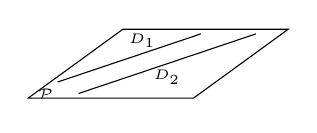
\begin{tikzpicture}  % ------ Deux droites parallèles dans un plan -------
      [x={(-0.572cm,-0.416cm)},y={(1cm,0cm)},z={(0cm,1cm)}, scale=.7]
\begin{tiny}        
    \coordinate (P1) at (0,0,0);    
    \coordinate (P2) at (0,3,0);
    \coordinate (P3) at (3,3,0);  
    \coordinate (P4) at (3,0,0);  
    \coordinate (A) at (1,.5,0); 
    \coordinate (B) at (2,2,0); 
    \coordinate (C) at (.5,2.5,0); 
    \coordinate (L) at (2,4,0); 
    

    \draw (P1)  -- (P2)  -- (P3) -- (P4) -- cycle  ; 
  \draw  (1.5,1.66,0) node [below] {$D_2$} ;  \draw  (.5,1,0) node  [left] {$D_1$}  ; 
    \draw (.2,1.53,0)   -- (2.3,0.133,0);  % (D1)  = (-2/3)x +(5/3) 
    \draw (.2,2.53,0)-- (2.8,.8,0) ;  % (D2)  = (-2/3)x +(8/3)  
    \draw (2.8,.2,0) node {$\mathcal{P}$} ;
\end{tiny}    
\end{tikzpicture} &
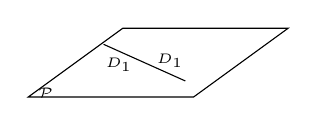
\begin{tikzpicture}  % ------ Droites confondues dans un plan -----------
      [x={(-0.572cm,-0.416cm)},y={(1cm,0cm)},z={(0cm,1cm)}, scale=.7]
\begin{tiny}        
    \coordinate (P1) at (0,0,0);    
    \coordinate (P2) at (0,3,0);
    \coordinate (P3) at (3,3,0);  
    \coordinate (P4) at (3,0,0);  
    \coordinate (A) at (1,.5,0); 
    \coordinate (B) at (2,2,0); 
    \draw (P1)  -- (P2)  -- (P3) -- (P4) -- cycle  ; 
    \draw  (A) node [below] {$D_1$} ; \draw (B)  node [above ]  {$D_1$} ; 
    \draw (.7,.05,0) -- (2.3,2.45,0)  ; % (AB) 1.5x -1 
    \draw (2.8,.2,0) node {$\mathcal{P}$} ;
\end{tiny}    
\end{tikzpicture} &
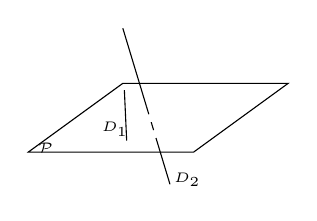
\begin{tikzpicture}  % ------ 2 droites non coplanaires -------------------
      [x={(-0.572cm,-0.416cm)},y={(1cm,0cm)},z={(0cm,1cm)}, scale=.7]
\begin{tiny}        
    \coordinate (P1) at (0,0,0);    
    \coordinate (P2) at (0,3,0);
    \coordinate (P3) at (3,3,0);  
    \coordinate (P4) at (3,0,0);  
    \coordinate (A) at (1,.5,0); 
    \coordinate (B) at (2,2,0); 
    \draw (P1)  -- (P2)  -- (P3) -- (P4) -- cycle  ; 
     \draw  (2,1,0) node {$D_1$} ; \draw  (1.8,2.2,-1) node  {$D_2$}  ; 
    \draw (2.5,1.5,0) -- (.3,.2,0)  ; % (AB) 1.5x -2 
    \draw (0,0,1) -- (1,1,0) ;   
    \draw [dashed] (1,1,0) -- (1.5,1.5,-.5) ;  
    \draw  (1.5,1.5,-.5)  -- (2,2,-1) ;      
    \draw (2.8,.2,0) node {$\mathcal{P}$} ;
\end{tiny}    
\end{tikzpicture} \\
\multicolumn{1}{c}{} &
       \multicolumn{1}{c}{$D_1$ et $D_2$} &
              \multicolumn{1}{c}{$D_1$ et $D_2$}  & \multicolumn{1}{c}{}\\
\multicolumn{1}{c}{} & \multicolumn{1}{c}{sont strictement } &
              \multicolumn{1}{c}{sont}  & \multicolumn{1}{c}{}\\
\multicolumn{1}{c}{} & \multicolumn{1}{c}{parallèles} &
              \multicolumn{1}{c}{confondues}  & \multicolumn{1}{c}{}\\                            
\end{tabular}
\end{center}

\textbf{Exemple} \\

%Dessin
\begin{center}
\begin{tabular}{cl}
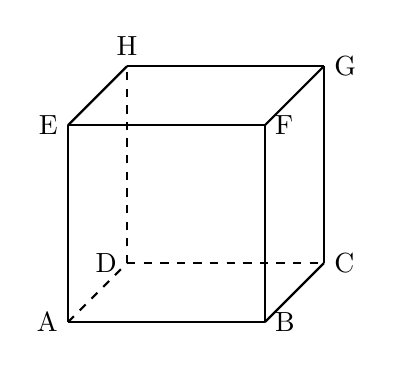
\begin{tikzpicture}[thick,scale=2.5]
    \coordinate (A1) at (0, 0);
    \coordinate (A2) at (0, 1);
    \coordinate (A3) at (1, 1);
    \coordinate (A4) at (1, 0);
    \coordinate (B1) at (0.3, 0.3);
    \coordinate (B2) at (0.3, 1.3);
    \coordinate (B3) at (1.3, 1.3);
    \coordinate (B4) at (1.3, 0.3);

    \draw (A1) node [left] {A} -- (A2)node [left] {E};
    \draw (A2)  -- (A3) node [right] {F} ;
    \draw (A3) -- (A4)  node [right] {B};
    \draw (A4) -- (A1);

    \draw[dashed] (A1) -- (B1) node [left] {D} ;
    \draw[dashed] (B1) -- (B2) node [above] {H};
    \draw (A2) -- (B2);
    \draw (B2) -- (B3) node [right] {G};
    \draw (A3) -- (B3);
    \draw (A4) -- (B4) node [right] {C};
    \draw (B4) -- (B3);
    \draw[dashed] (B1) -- (B4);

\end{tikzpicture} & \raisebox{10ex}{\parbox{8cm}{
 \begin{itemize}
  \setlength{\itemsep}{1.4mm}
     \item [] $\left(EG\right)$ et $(CG)$ sont  ? $\qquad$   {\cursive  sécantes en } G.
    \item [] $(AD)$ et $(FG)$ sont ? $\qquad$  {\cursive parallèles}.
  \setlength{\itemsep}{0mm}
    \item []  $ (EH)$ et $(GC)$ sont ? $\qquad$  {\cursive non-coplanaires}.
\end{itemize}
}}\\
\end{tabular}
\end{center}



\subsubsection{Position relative de 2 plans}

%Dessin
\begin{center}
\begin{tabular}{ccc}
\multicolumn{1}{c}{$\mathcal{P}_1$ et $\mathcal{P}_2$ sécants } & 
    \multicolumn{2}{c}{$\mathcal{P}_1$ et $\mathcal{P}_2$ parallèles} \\
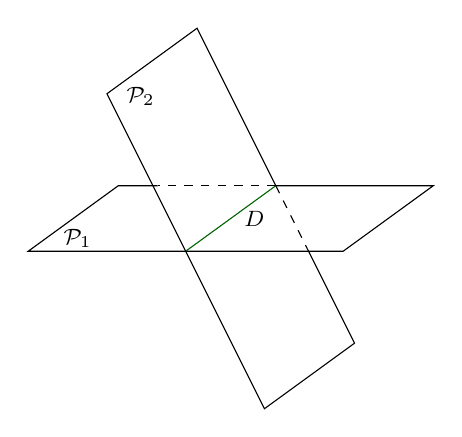
\begin{tikzpicture}  % ------ Plans secants -------------------
      [x={(-0.572cm,-0.416cm)},y={(1cm,0cm)},z={(0cm,1cm)},scale=1]
    \coordinate (A1) at (0,4,0);
    \coordinate (A2) at (0,0,0);
    \coordinate (A3) at (2,0,0);
    \coordinate (A4) at (2,4,0);`
    \coordinate (M1) at (0,2,0);
    \coordinate (M2) at (2,2,0);
    

    \coordinate (B1) at (2,3,-2);`
    \coordinate (B2) at (2,1,2);
    \coordinate (B3) at (0,1,2);
    \coordinate (B4) at (0,3,-2);

    \draw [dashed] (M1) -- (0,.5,0)  ; 
    \draw (0,.5,0)  -- (A2) -- (A3) -- (A4) -- (A1) -- (M1)  ; 
    \draw [DarkGreen] (M1) -- (M2) ;  
    \draw [dashed] (M1) -- (0,2.4,-.8)  ;  
    \draw (0,2.4,-.8)  -- (B4) -- (B1) -- (B2) -- (B3) -- (M1) ;     
\begin{footnotesize}
    \draw (1.6,.4,0) node {$\mathcal{P}_1$} ; 
    \draw (1.6,1.2,1.8) node {$\mathcal{P}_2$} ; 
    \draw (1,2.3,0) node {$D$} ;        
\end{footnotesize}          
\end{tikzpicture} &
\raisebox{10ex}{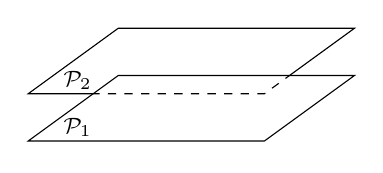
\begin{tikzpicture}  % ------ Plans parallèles ---------------
      [x={(-0.572cm,-0.416cm)},y={(1cm,0cm)},z={(0cm,1cm)},scale=1]
    \coordinate (A1) at (0,3,0);
    \coordinate (A2) at (0,0,0);
    \coordinate (A3) at (2,0,0);
    \coordinate (A4) at (2,3,0);`

    \coordinate (B1) at (0,3,.6);`
    \coordinate (B2) at (0,0,.6);
    \coordinate (B3) at (2,0,.6);
    \coordinate (B4) at (2,3,.6);

    \draw (A1) -- (A2) -- (A3) -- (A4) -- cycle ; 
    \draw (1.4,3,.6) -- (B1) -- (B2) -- (B3) -- (2,.8,.6)  ;  
    \draw [dashed] (2,.8,.6) -- (B4) -- (1.4,3,.6)  ;   
\begin{footnotesize}
    \draw (1.6,.4,0) node {$\mathcal{P}_1$} ; 
    \draw (1.6,.4,.6) node {$\mathcal{P}_2$} ;     
\end{footnotesize}          
\end{tikzpicture}} & 
\raisebox{12ex}{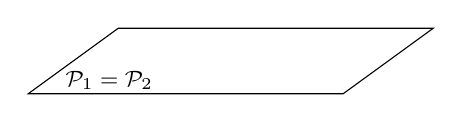
\begin{tikzpicture}  % ------ Plans confondus --------------
      [x={(-0.572cm,-0.416cm)},y={(1cm,0cm)},z={(0cm,1cm)},scale=1]
    \coordinate (A1) at (0,4,0);
    \coordinate (A2) at (0,0,0);
    \coordinate (A3) at (2,0,0);
    \coordinate (A4) at (2,4,0);
 
    \draw (A1) -- (A2) -- (A3)  -- (A4) -- cycle ;     
\begin{footnotesize}
    \draw (1.6,.8,0) node {$\mathcal{P}_1=\mathcal{P}_2$} ;        
\end{footnotesize}          
\end{tikzpicture}}\\
\multicolumn{1}{c}{$\mathcal{P}_1 \cap \mathcal{P}_2 = D$} &
    \multicolumn{1}{c}{$\mathcal{P}_1 \cap \mathcal{P}_2 = \varnothing$} &
        \multicolumn{1}{c}{$\mathcal{P}_1 \cap \mathcal{P}_2 = \mathcal{P}_1 = \mathcal{P}_2$} \\
\end{tabular}
\end{center}
      
\textbf{Exemple}

%Refaire le dessin du cube, et tracer en pointillés le plan (ABH) et le plan (EFC)
\begin{center}

\begin{tabular}{cl}
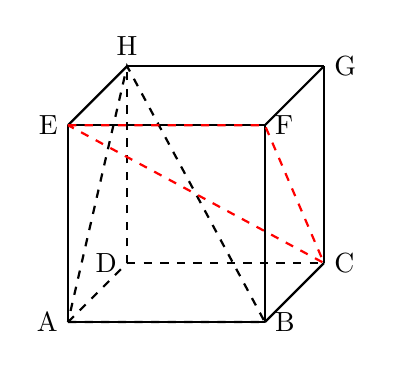
\begin{tikzpicture}[thick,scale=2.5]
    \coordinate (A1) at (0, 0);
    \coordinate (A2) at (0, 1);
    \coordinate (A3) at (1, 1);
    \coordinate (A4) at (1, 0);
    \coordinate (B1) at (0.3, 0.3);
    \coordinate (B2) at (0.3, 1.3);
    \coordinate (B3) at (1.3, 1.3);
    \coordinate (B4) at (1.3, 0.3);

    \draw (A1) node [left] {A} -- (A2)node [left] {E};
    \draw (A2)  -- (A3) node [right] {F} ;
    \draw (A3) -- (A4)  node [right] {B};
    \draw (A4) -- (A1);

    \draw[dashed] (A1) -- (B1) node [left] {D} ;
    \draw[dashed] (B1) -- (B2) node [above] {H};
    \draw (A2) -- (B2);
    \draw (B2) -- (B3) node [right] {G};
    \draw (A3) -- (B3);
    \draw (A4) -- (B4) node [right] {C};
    \draw (B4) -- (B3);
    \draw[dashed] (B1) -- (B4);
    
    \draw [dashed] (A1) --  (A4) --  (B2) -- cycle ; % (ABH) 
    \draw [dashed, red] (A2) -- (A3) -- (B4) -- cycle ; % (EFC) 
    

\end{tikzpicture} & \raisebox{10ex}{\parbox{8cm}{
 \begin{itemize} \setlength{\itemsep}{1.4mm}
\item []  $(EFC)$ et $(FBC)$ sont ? {\cursive sécants suivant} (FG)\\
\item []  $(EFG)$ et $(AGH)$ sont ? {\cursive sécants suivant} (GH)\\
\item []  $(EFG)$ et $(ADC)$ sont ? {\cursive  parallèles}\\
\item []  $(EFC)$ et $(CDE)$ sont ? {\cursive confondus}
\end{itemize} }} \\
\end{tabular}
\end{center}

\subsubsection{Position relative d'une droite et d'un plan}

%dessin
\begin{center}
\begin{tabular}{ccc}
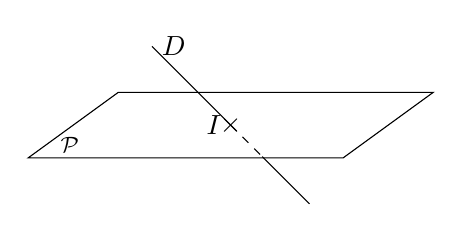
\begin{tikzpicture}  % ------ Plans percé  ---------------
      [x={(-0.572cm,-0.416cm)},y={(1cm,0cm)},z={(0cm,1cm)},scale=1]    
    \coordinate (A1) at (0,4,0);
    \coordinate (A2) at (0,0,0);
    \coordinate (A3) at (2,0,0);
    \coordinate (A4) at (2,4,0);
 
    \draw (A1) -- (A2) -- (A3)  -- (A4) -- cycle ;    
    \draw (1,1,1) node [right] {$D$}  -- (1,2,0) node {$\times$}  ; 
    \draw [dashed] (1,2,0) node [left] {$I$} -- (1,2.4,-.4) ; 
    \draw (1,2.4,-.4) -- ( 1, 3, -1) ; 
\begin{footnotesize}
    \draw (1.6,.3,0) node {$\mathcal{P}$} ;        
\end{footnotesize}                   
\end{tikzpicture} &
\raisebox{3.5ex}{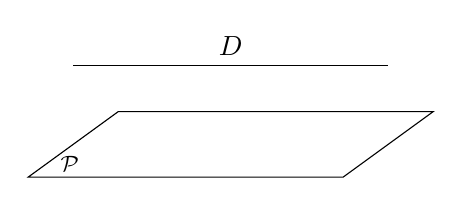
\begin{tikzpicture}  % ------ Parallèle au plan -----------
      [x={(-0.572cm,-0.416cm)},y={(1cm,0cm)},z={(0cm,1cm)},scale=1]
    \coordinate (A1) at (0,4,0);
    \coordinate (A2) at (0,0,0);
    \coordinate (A3) at (2,0,0);
    \coordinate (A4) at (2,4,0);
 
    \draw (A1) -- (A2) -- (A3)  -- (A4) -- cycle ; 
    \draw (1,0,1) -- node [midway, above] {$D$} (1,4,1) ; 
        
\begin{footnotesize}
    \draw (1.6,.3,0) node {$\mathcal{P}$} ;        
\end{footnotesize}                   
\end{tikzpicture}} & 
\raisebox{3.5ex}{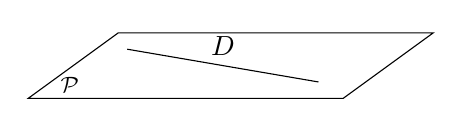
\begin{tikzpicture}  % ------ droite incluse  --------------
      [x={(-0.572cm,-0.416cm)},y={(1cm,0cm)},z={(0cm,1cm)},scale=1]
    \coordinate (A1) at (0,4,0);
    \coordinate (A2) at (0,0,0);
    \coordinate (A3) at (2,0,0);
    \coordinate (A4) at (2,4,0);
 
    \draw (A1) -- (A2) -- (A3)  -- (A4) -- cycle ; 
    \draw (.5,.4,0) -- node [midway, above] {$D$} (1.5,3.4,0) ; 
        
\begin{footnotesize}
    \draw (1.6,.3,0) node {$\mathcal{P}$} ;        
\end{footnotesize}          
\end{tikzpicture}}\\
\multicolumn{1}{c}{$D$ perce le plan } &
    \multicolumn{1}{c}{$D$ est parallèle à $\mathcal{P}$} &
        \multicolumn{1}{c}{$D$ est incluse dans $\mathcal{P}$} \\
        \multicolumn{1}{c}{$D \cap \mathcal{P} = \lbrace I\rbrace$ } &
    \multicolumn{1}{c}{$D \cap \mathcal{P} = \varnothing$ } &
        \multicolumn{1}{c}{$D \cap \mathcal{P} = D$ } \\
\end{tabular}
\end{center}
\subsection{Parallélisme dans l'espace}

\subsubsection{Droites parallèles à un plan}

\textbf{Propriété :} Si une droite $D$ est parallèle à une droite $\Delta$ contenue dans un plan $P$, alors $D$ est parallèle à $P$. \\

\bigskip 

\bigskip 

\bigskip 

\textbf{Théorème du toit}

%Dessin
\begin{center}
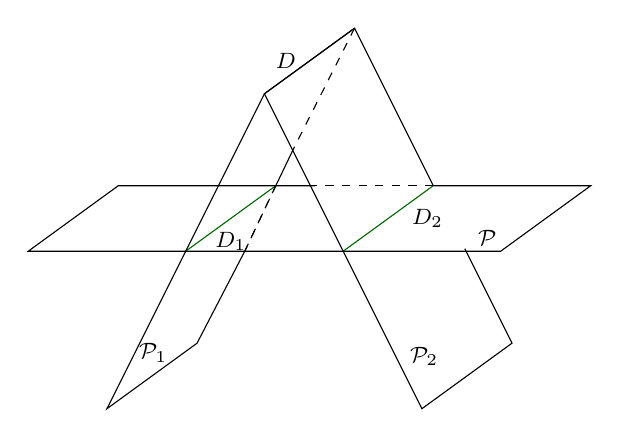
\begin{tikzpicture}  % ------ Théorème du toit -------------------
      [x={(-0.572cm,-0.416cm)},y={(1cm,0cm)},z={(0cm,1cm)},scale=1]
    \coordinate (A1) at (0,4,0);
    \coordinate (A2) at (0,-2,0);
    \coordinate (A3) at (2,-2,0);
    \coordinate (A4) at (2,4,0);`
    \coordinate (M1) at (0,2,0);
    \coordinate (M2) at (2,2,0);
    \coordinate (M3) at (0,0,0);
    \coordinate (M4) at (2,0,0);
    \coordinate (M5) at (.3,.4,.6);
    
    \coordinate (B1) at (2,3,-2);`
    \coordinate (B2) at (2,1,2);
    \coordinate (B3) at (0,1,2);
    \coordinate (B4) at (0,3,-2);
    
    \coordinate (C1) at (2,-1,-2);
    \coordinate (C2) at (2,1,2);
    \coordinate (C3) at (0,1,2);
    \coordinate (C4) at (0,-1,-2);

    \draw [dashed] (M1) -- (0,.5,0)  ; 
    \draw (0,.5,0)  -- (A2) -- (A3) -- (A4) -- (A1) -- (M1)  ; 
    \draw [DarkGreen] (M1) -- (M2) ;  
    \draw [DarkGreen] (M3)  -- (M4) ; 
    
    \draw [dashed] (C3) -- (M5);
    \draw (M5)  -- (M3) ;  
    \draw (0,2.4,-.8)  -- (B4) -- (B1) -- (B2) -- (B3) -- (M1) ;     
    
    \draw [dashed] (2,.75,0)-- (M3)  ;
    \draw [dashed] (M3) -- (2,.75,0)  ;
    \draw (2,.75,0) -- (C4)  -- (C1)-- (C2)  -- (C3); 
      
\begin{footnotesize}
   \draw (1.5,-.7,-1.5) node {$\mathcal{P}_1$} ;     
   \draw (1.6,2.8,-1.5) node {$\mathcal{P}_2$} ; 
   \draw (1.6,3.6,0) node {$\mathcal{P}$} ; 
   \draw (1.7,.4,0) node {$D_1$} ;
   \draw (1,2.5,0) node {$D_2$} ;       
   \draw (1,.7,2) node {$D$} ;       
\end{footnotesize}          
\end{tikzpicture} 
\end{center}


On a : $D_1 // D_2$. $D_1 \subset P_1$ et $D_2 \subset P_2$.

$P_1$ et $P_2$ sont sécants suivants $D$, donc $D$ est parralèle à $D_1$ et $D_2$.

\newpage

\subsubsection{Plans parallèles}

\textbf{Propriété n°1 :} Si un plan contient deux droites $D_1$ et $D_2$ sécantes et parallèles à un plan $P'$, alors $P$ est parallèle à $P'$.

\bigskip 

\bigskip

\bigskip 


\textbf{Propriété n°2 :} 

\begin{center}
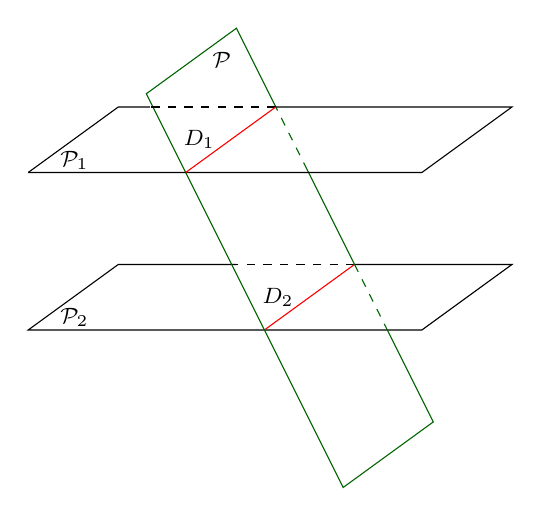
\begin{tikzpicture}  % --- plan sécant à 2 plans parallèles -----------
      [x={(-0.572cm,-0.416cm)},y={(1cm,0cm)},z={(0cm,1cm)},scale=1]
    \coordinate (A1) at (0,4,0);
    \coordinate (A2) at (0,-1,0);
    \coordinate (A3) at (2,-1,0);
    \coordinate (A4) at (2,4,0);
    
    \coordinate (M1) at (0,2,0);
    \coordinate (M2) at (2,2,0);
    \coordinate (M3) at (0,1,2);
    \coordinate (M4) at (2,1,2);
%    \coordinate (M5) at (.3,.4,.6);
    
    \coordinate (B1) at (2,3,-2);`
    \coordinate (B2) at (2,.5,3);
    \coordinate (B3) at (0,.5,3);
    \coordinate (B4) at (0,3,-2);
    
    \coordinate (C1) at (0,4,2);
    \coordinate (C2) at (0,-1,2);
    \coordinate (C3) at (2,-1,2);
    \coordinate (C4) at (2,4,2);

    \draw [dashed] (M1) -- (0,.5,0)  ; 
    \draw (0,.5,0)  -- (A2)  -- (A3)  -- (A4)  -- (A1) -- (M1)  ; 
    \draw [red] (M1) -- (M2) ;  

    \draw [DarkGreen] (M1) -- (0,1.4,1.2)  ;
    \draw [dashed,DarkGreen] (M1) -- (0,2.4,-.8)  ; 
    \draw [dashed, DarkGreen] (0,1.4,1.2) -- (M3)  ;     
    \draw [DarkGreen] (0,2.4,-.8)  -- (B4)  -- (B1)  -- (B2) -- (B3) -- (M3) ;     
     
    \draw  (0,-.6,2)-- (C2)  -- (C3)  ; 
    \draw [dashed] (M3) -- (0,-.6,2)  ; 
    \draw   (C3) -- (C4)-- (C1) -- (M3)  ; 
    \draw [red] (M3) -- (M4) ;
         
\begin{footnotesize}
  \draw (1.5,-.7,1.95) node {$\mathcal{P}_1$} ;     
  \draw (1.5,-.7,-.05) node {$\mathcal{P}_2$} ; 
  \draw (0.5,0.6,2.8) node {$\mathcal{P}$} ; 
  \draw (1,.6,2) node {$D_1$} ;
  \draw (1,1.6,0) node {$D_2$} ;            
\end{footnotesize}          
\end{tikzpicture} 
\end{center}

Si deux plans $P_1$ et $P_2$ sont parallèles, alors tout plan $P$ sécant à $P_1$ est sécant à $P_2$ et les droites d'intersection $D_1$ et $D_2$ sont parallèles.